\documentclass[border=15pt, multi, tikz]{article}
\usepackage[backend=bibtex,style=authoryear,natbib=true]{biblatex} % Use the bibtex backend with the authoryear citation style (which resembles APA)

\addbibresource{example.bib} % The filename of the bibliography

\usepackage[autostyle=true]{csquotes} % Required to generate language-dependent quotes in the bibliography



\usepackage{amssymb}
\usepackage[backend=bibtex,style=authoryear,natbib=true]{biblatex} % Use the bibtex backend with the authoryear citation style (which resembles \left( APA)

\addbibresource{example.bib} % The filename of the bibliography

\usepackage[autostyle=true]{csquotes} % Required to generate language-dependent quotes in the bibliography
\usepackage{import}
\usepackage{float}
\usepackage{tikz}
\usepackage{tikz-network}
\usepackage{breqn}
\usepackage{bm}
\usepackage{graphicx}
\usepackage{subcaption}
\usepackage{multirow}
\usepackage{pdfpages}
\usepackage{pgfplots}
\usepackage{rotating}
\usetikzlibrary{fit}
\usetikzlibrary{calc,patterns,angles,quotes}
\usetikzlibrary {arrows.meta,graphs,shapes.misc}
\usetikzlibrary {positioning}

\usepackage{tikz-3dplot}
\usetikzlibrary{calc}
\newcommand{\DrawPlane}[3][]{\draw[#1] 
	(-1*\PlaneScale,{\PlaneScale*cos(#2)},{\PlaneScale*sin(#2)})
	-- ++  (2*\PlaneScale,0,0)
	-- ++ (0,{sqrt(3)*\PlaneScale*cos(#3)},{sqrt(3)*\PlaneScale*sin(#3)})
	-- ++  (-2*\PlaneScale,0,0) -- cycle;}
\newcommand{\DrawSinglePlane}[2][]{\ifcase#2
	\or
	\DrawPlane[fill=blue,#1]{210}{240} %left bottom 
	\or
	\DrawPlane[fill=red,#1]{-30}{-60} % right bottom
	\or
	\DrawPlane[fill=purple,#1]{210}{180} % bottom left
	\or
	\DrawPlane[fill=purple,#1]{210}{0} % bottom middle
	\or
	\DrawPlane[fill=purple,#1]{-30}{0} % bottom right
	\or
	\DrawPlane[fill=blue,#1]{90}{240} % left top
	\or
	\DrawPlane[fill=red,#1]{90}{-60} % right middle
	\or
	\DrawPlane[fill=red,#1]{90}{120} % right top
	\or
	\DrawPlane[fill=blue,#1]{90}{60} % left top
	\fi
} 

\usetikzlibrary{fit}
\usetikzlibrary {arrows.meta,graphs,shapes.misc}
\usetikzlibrary {positioning}
\subimport{./layers/}{init}
\newcommand{\bn}{\textbf{n}}
\newcommand{\tabhead}[1]{\textbf{#1}}

\def\ConvColor{rgb:yellow,5;red,2.5;white,5}
\def\ConvReluColor{rgb:yellow,5;red,5;white,5}
\def\PoolColor{rgb:red,1;black,0.3}
\def\DcnvColor{rgb:blue,5;green,2.5;white,5}
\def\SoftmaxColor{rgb:magenta,5;black,7}
\def\SumColor{rgb:blue,5;green,15}
\def\poolsep{1}


\begin{document}
\begin{figure}[h!]
	\centering
	\tdplotsetmaincoords{70}{110}
	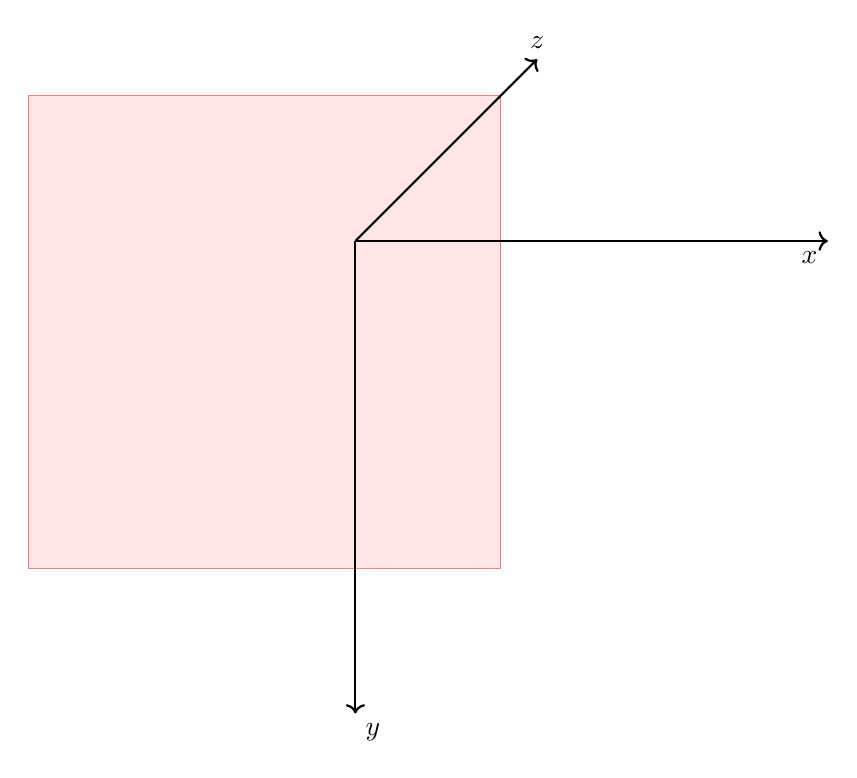
\begin{tikzpicture} [scale=3]	
		% reference lines
%		\node[inner sep=10pt] (input) at (0,0)
%		{\includegraphics[width=\linewidth]{./Figures/ply_config.png}};

\filldraw[
draw=red,%
fill=red!20,%
opacity=0.5,
]  (1,1,1)
-- (1,-1,1)
-- (-1,-1,1)
-- (-1,1,1)
-- cycle;
\draw[thick,->] (0,0,0) -- (2,0,0) node[anchor=north east]{$x$};

\draw[thick,->] (0,0,0) -- (0,-2,0) node[anchor=north west]{$y$};
\draw[thick,->] (0,0,0) -- (0,0,-2) node[anchor=south]{$z$};
%		\draw[thick,dashed]	(0,0) -- (10,0) ; % bottom
%		\draw[thick,dashed]	(0,3) -- (10,3) node[pos=0.9, above] {image plane}; % middle
%		\draw[thick,dashed]	(0,6) -- (10,6); % top
		% camera 
%		\filldraw[black] (5,0) circle (2pt) node[anchor=south west]{Camera Position};
		% world point 
%		\filldraw[black] (2,2) circle (2pt) node[anchor=north west]{Point};
		% image point
%		\filldraw[black] (6,3) circle (2pt) node[anchor=north west]{Pixel};
		% similiar triangles
%		\draw[thick] (0,0) -- (2,6); % AB
%		\draw[thick] (5,0) -- (7,6); % AC
%		\draw[thick] (5,6) -- (7,6) node[midway, below] {$ X $}; % BC
%		\draw[thick] (5,3) -- (6,3) node[midway, below] {$ u $};
%		% measure arrows
%		\draw[thick, <->] (4,0) -- (4,3) node[midway, left] {$ fk_u $};
%		\draw[thick, <->] (3,0) -- (3,6) node[pos=0.3, left] {$ Z $};
	\end{tikzpicture}	
	\caption{Data Collection configuration}
	\label{fig:depth-triangulation}
\end{figure}


\end{document}
